\begin{acronym}
	\acro{p2p}[P2P]{peer-to-peer}
	\acro{lww}[LWW]{last-write-wins}
	\acro{json}[JSON]{JavaScript Object Notation}
	\acro{ecs}[ECS]{external configuration service}
	\acro{fifo}[FIFO]{first-in-first-out}
	\acro{lru}[LRU]{least-recently-used}
	\acro{lfu}[LFU]{least-frequently-used}
	\acro{wal}[WAL]{write-ahead-log}
	\acro{lsm}[LSM]{log-structured-merge-tree}
	\acro{api}[API]{application programmer interface}
	\acro{utf8}[UTF-8]{8-Bit Univeral Character Set Transformation Format}
	\acro{cli}[CLI]{command-line interface}
\end{acronym}

\section{Motivation}
In 2017, the total retail sales volume in the US equalled \$3,496 billion \cite{Ali2018} and it grows year by year.
An ever increasing fraction of the total volume can be attributed to eCommerce.
Amazon's Prime service has shipped 5 billion items in 2017 \cite{Carman2018}.
Alibaba reports to process 325,000 orders per second \cite{Fenol2018} in the same year.

Assuming an average order record is about 3kB in size\footnote{Estimated based on the online retail data set described in \cite{Chen2012}.},
this translates into 1GB of new data being produced every second.
Traditional relational databases that employ normalized storage schemes and provide advanced
features like complex querying and multi-document transactions have problems scaling to such levels.

This problem gave rise to a new type of technology, the so-called \emph{NoSQL} databases~\cite{Kleppmann2017}.
These leverage the fact that many types of data are accessed on document-level and a simple lookup by primary ID is sufficient.
In return they make it easy to partition data across many nodes and are highly scalable by nature.%\\[1em]

Storing such data often is a legal requirement, but it also is incredibly valuable.
It is a vital ingredient to answer questions like which customers and products
are most valuable to the business, how do customers navigate the site, how marketing
campains should be designed, etc (cf.~\cite{Chen2012}).
Some people nowadays go as far as calling data the oil of the 21st century.

Amazon e.g. is known to change product prices up to 2.5 million times a day,
thereby increasing their sales by up to 25\%~\cite{Mehta2018}.
It is however not only important that these questions can be answered, but they have to be
answered as quickly as possible to reap the optimal benefits.
\\[1em]
The work at hand presents \emph{G4DB}, a highly scalable and failure-tolerant key-value-datastore 
with integrated MapReduce processing capabilities.
It handles the data volumes present in current retail settings and allows users
to run analyses directly on the stored data, thereby eliminating the latency involved
by the need of moving it to external systems.

The structure of this report is as follows.
Section~\ref{sec:related-work} talks about related work which has influenced our design.
Section~\ref{sec:approach} summarizes the key points of the G4DB design.
Section~\ref{sec:implementation} highlights some interesting implementation details.
Section~\ref{sec:evaluation} presents some performance metrics validating our design.
Section~\ref{sec:conclusion} finally concludes this work and introduces some avenues for future work on G4DB.
% TODO add structure?

\section{Related Work}
\label{sec:related-work}
A significant amount of work has been done in the area of scalable key-value-stores.
In 2006, a team of Google engineers designed \emph{BigTable}~\cite{Chang2006},
a distributed datastore to power their websearch.
BigTable is built upon other services: data is stored in
Google's distributed fileystem (GFS) and coordination is implemented using
a highly-consistent external configuration service (Chubby).
BigTable clusters are coordinated by a single master that has to be recovered
in a time-consuming procedure in failure cases.

\emph{Dynamo}~\cite{DeCandia2007} was designed by Amazon in 2007 as
distributed datastore backing the shopping cart system.
In contrast to BigTable, Dynamo is a self-contained system, i.e. it does not rely on other services.
Instead of relying on a single master node for coordination, Dynamo implements a
Gossip-based membership coordination mechanism.
Dynamo aims at always accepting writes, at the cost of forcing readers to
do conflict resolution.
The idea is that users can easily remove things from their shopping carts again
if they should appear due to conflicts.

\emph{Gossiping} is a \ac{p2p} mechanism with the goal of broadcasting information
to a number of nodes without the need of having pair-wise communication channels
between nodes (which would imply factorial growth).
Early work on using Gossip mechanisms for coordination of disitributed
databases dates back to Alan Demers and colleagues in Xerox PARC in 1989~\cite{Demers1987},
but Dynamo is the first work to validate the approach with modern web-scale software
to the authors' knowledge.

In 2010, \emph{Cassandra}~\cite{Lakshman2010} has been developed at Facebook.
Cassandra is very similar to Dynamo, but moves the responsibility of resolving
conflicts back to the server using a simple \ac{lww} strategy.
It has been open-sourced and there are many companies operating Cassandra clusters,
one of the largest being Apple with 75,000 nodes and 10PB of data~\cite{Cassandra}.

A major contribution to the field of distributed data processing was
Google's works on \emph{MapReduce}~\cite[]{Dean2008}.
It has been found to provide a powerful abstraction for writing
distributed and failure-tolerant data processing software.
MapReduce has been implemented in many open source products such as
Apache~Hadoop~\cite[]{Hadoop} and Apache~Spark~\cite[]{Zaharia2014}.
It is one of the defining technologies for the "BigData" industry.

There are some datastores with integrated MapReduce-engines, the best
known ones likely being \emph{MongoDB}~\cite[]{MongoDB} and \emph{CouchDB}~\cite[]{CouchDB}.    

\section{Approach}
\label{sec:approach}

This section describes the cornerstones of G4DB's design with regards to
scalability, failure-tolerance and efficient processing of large amounts
of data.

The working assumptions are as follows:
\begin{enumerate}
	\item Both read and write workloads must be reasonably performant.
		Appending new data should not be unnecessarily blocked by
		current read operations.
	\item Data should not be lost, temporary inconsistencies for single items are
		OK.
	\item The system will encounter big and varying volumes of data and should
		be able to scale accordingly.
	\item With regard to failure-tolerance and scalability, the need for
		central coordinators should be reduced as much as possible.
	\item Data should not have to be moved to do analytical processing
		in order to reduce latency.
\end{enumerate}

Due to the limited amount of space, we focus on the concepts of \emph{partitioning},
\emph{replication}, \emph{membership coordination} and \emph{MapReduce}-processing.   
The first three modules collaborate closely to handle read/write requests.
A client initially connects to an arbitrary node in the G4DB cluster and
sends requests to this node.
The node knows about the whole cluster and determines if it is responsible for the
request.
If it is responsible, it persists the data and queues it up for replication.
Replication happens completely asynchronously, so there can be periods of time
where different replicas return different values for a key (eventual consistency).
If it is not responsible, it sends the cluster information to the client.
The client then redirects its request to the correct node.

\subsection{Data Model}

The data model of G4DB are simple key-value-tuples; both key and value are \acs{utf8}-encoded strings.
The client is responsible for encoding/decoding semi-structured data in an appropriate
format like \ac{json}.

\subsection{Partitioning}

\begin{figure}[]
	%\centering
	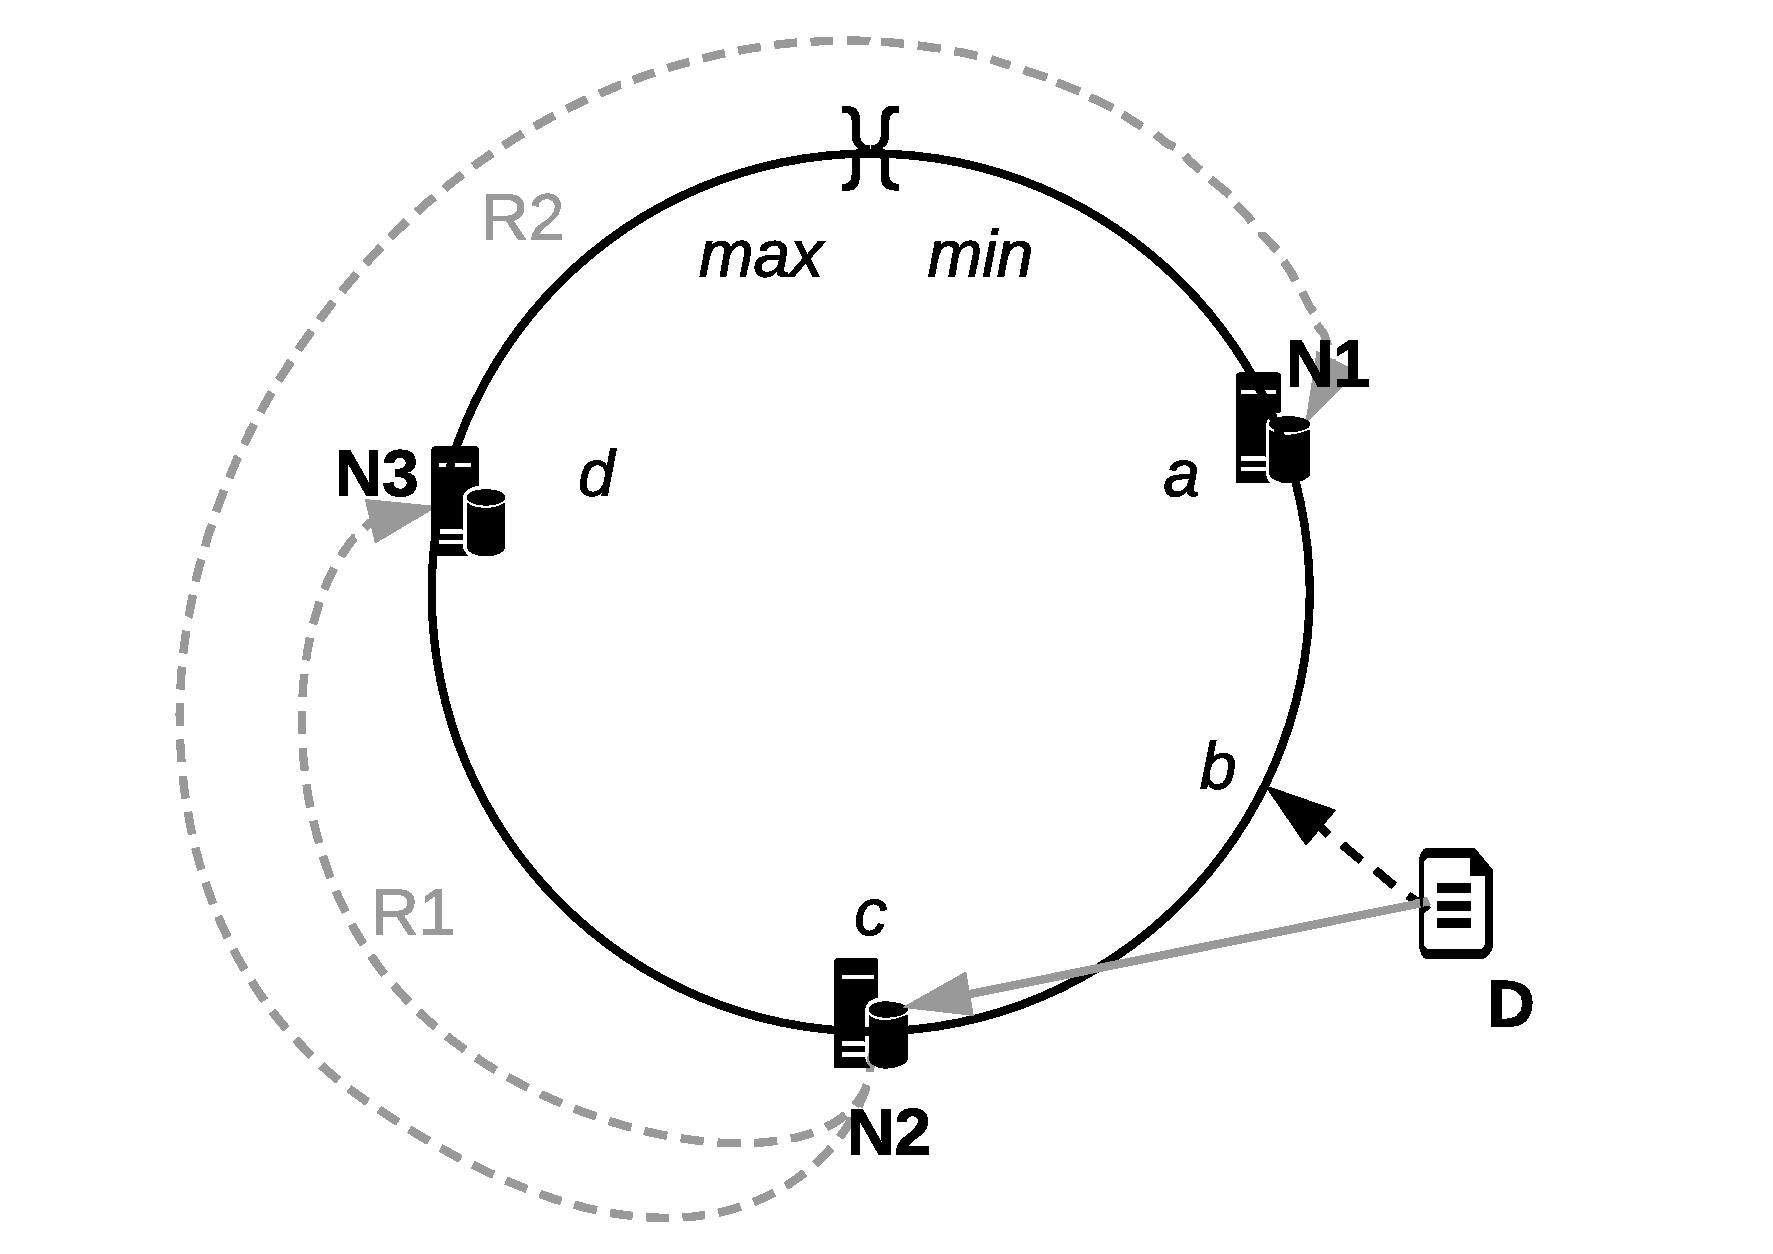
\includegraphics[width=0.4\textwidth]{resources/consistent-hashing-1}
	\caption{Consistent Hashing - Partitioning and Replication}
	\label{fig:consistent-hashing-partitioning}
	{
	Document $D$ is written to the database and hashes to position $b$.
	It therefore lies in the responsibility of node $N2$, since
	$b \in \resp(N2) = (a,c]$.
	With a replication factor of 3, $D$ would also be replicated to nodes
	$N3$ and $N1$ which are the direct successors of $N2$.
	}
\end{figure}

Scalability in distributed datastores is achieved by \emph{partitioning} data across
multiple nodes (sometimes also called \emph{sharding}). 
G4DB's partitioning mechanism is based on \emph{consistent hashing}~\cite[]{Karger1997}.
Consistent hashing provides a mechanism to distribute a range of keys across
a number of nodes such that only the close neighbors are impacted when we add or remove nodes.
This is important since we want to scale G4DB clusters incrementally without having
to move more data over the network than absolutely necessary.


The idea of consistent hashing is mapping
both the set of node addresses $\mathcal{N}$ and the set of keys $\mathcal{K}$
onto the same linear space $\mathcal{H} = [min,max]$
using a hash function $h: \mathcal{N} \cup \mathcal{K} \mapsto \mathcal{H}$.
This range is treated as a ring, i.e. the largest value wraps around to the smallest value.
A node $n$ is responsible for all keys which are hashed into the
range $\resp(n) = (h(n-1),h(n)]$, where $n$ denotes the position on the ring (cf.~Figure~\ref{fig:consistent-hashing-partitioning}).

Consistent hashing in this basic form creates some challenges regarding
uniform load distribution with a smaller number of nodes.
One way to approach this would be representing each physial node by several
virtual nodes that hash to different positions on the ring.

\subsection{Replication}

G4DB replicates data to 2 other nodes, thereby ensuring that two nodes can fail without data
being lost.
Consistent hashing provides a natural solution to coordinate replication:
assuming a desired replication factor of 3, all keys that are stored on node $n$ are replicated
to nodes $n+1$ and $n+2$.
The replication factor of 3 is currently fixed, but could be made configurable in future
developments.

\subsection{Membership}

Each G4DB node must know all the other cluster nodes in order to determine
for which data it is responsible so that it can handle requests correctly
and communicate to clients where requests should go.
When a node joins or leaves the cluster, the ranges of data for which its neighbors
are responsible changes and must possibly be transferred from other nodes.

In a centralized implementation, an \ac{ecs} would be responsible for coordinating
such processes.
However this \ac{ecs} would be a bottleneck given an
increasing number of nodes it has to communicate with.
\ac{p2p} mechanisms like Gossip-broadcasting allow the nodes to handle this process
amongst themselves in a more robust and scalable fashion.
G4DB still uses an \ac{ecs} as interface
for system admninistrators, but this service is responsible only for bootstrapping
and hands of further coordination work to the cluster as much as possible.

Gossip-based membership coordination works as follows.
Each node in the cluster maintains its own view of the current cluster composition.
The coordination takes place in rounds that are triggered by all nodes on a fixed schedule.
During a round, the initiating node randomly chooses a small number of peers.
It then exchanges its data with each of these peers, such that each party
has the more recent data of the other party after the exchange.
In the next round, new peers are chosen and the process is repeated with the updated state.
With every round more nodes learn the updated information until at some point all nodes have received it.

The advantage of Gossiping is that it scales to a huge number of nodes without
a factorial explosion in the number of communication paths.
The disadvantage is that it is hard to reason about when all the nodes in the cluster
will have converged to the same state.

Practical experiences with Dynamo and Cassandra have proven the suitability of this mechanism.
We present some simulations for our implementation in Section~\ref{sec:implementation:gossip:peers}.

\subsubsection{Adding Nodes}

\begin{figure}[]
	\centering
	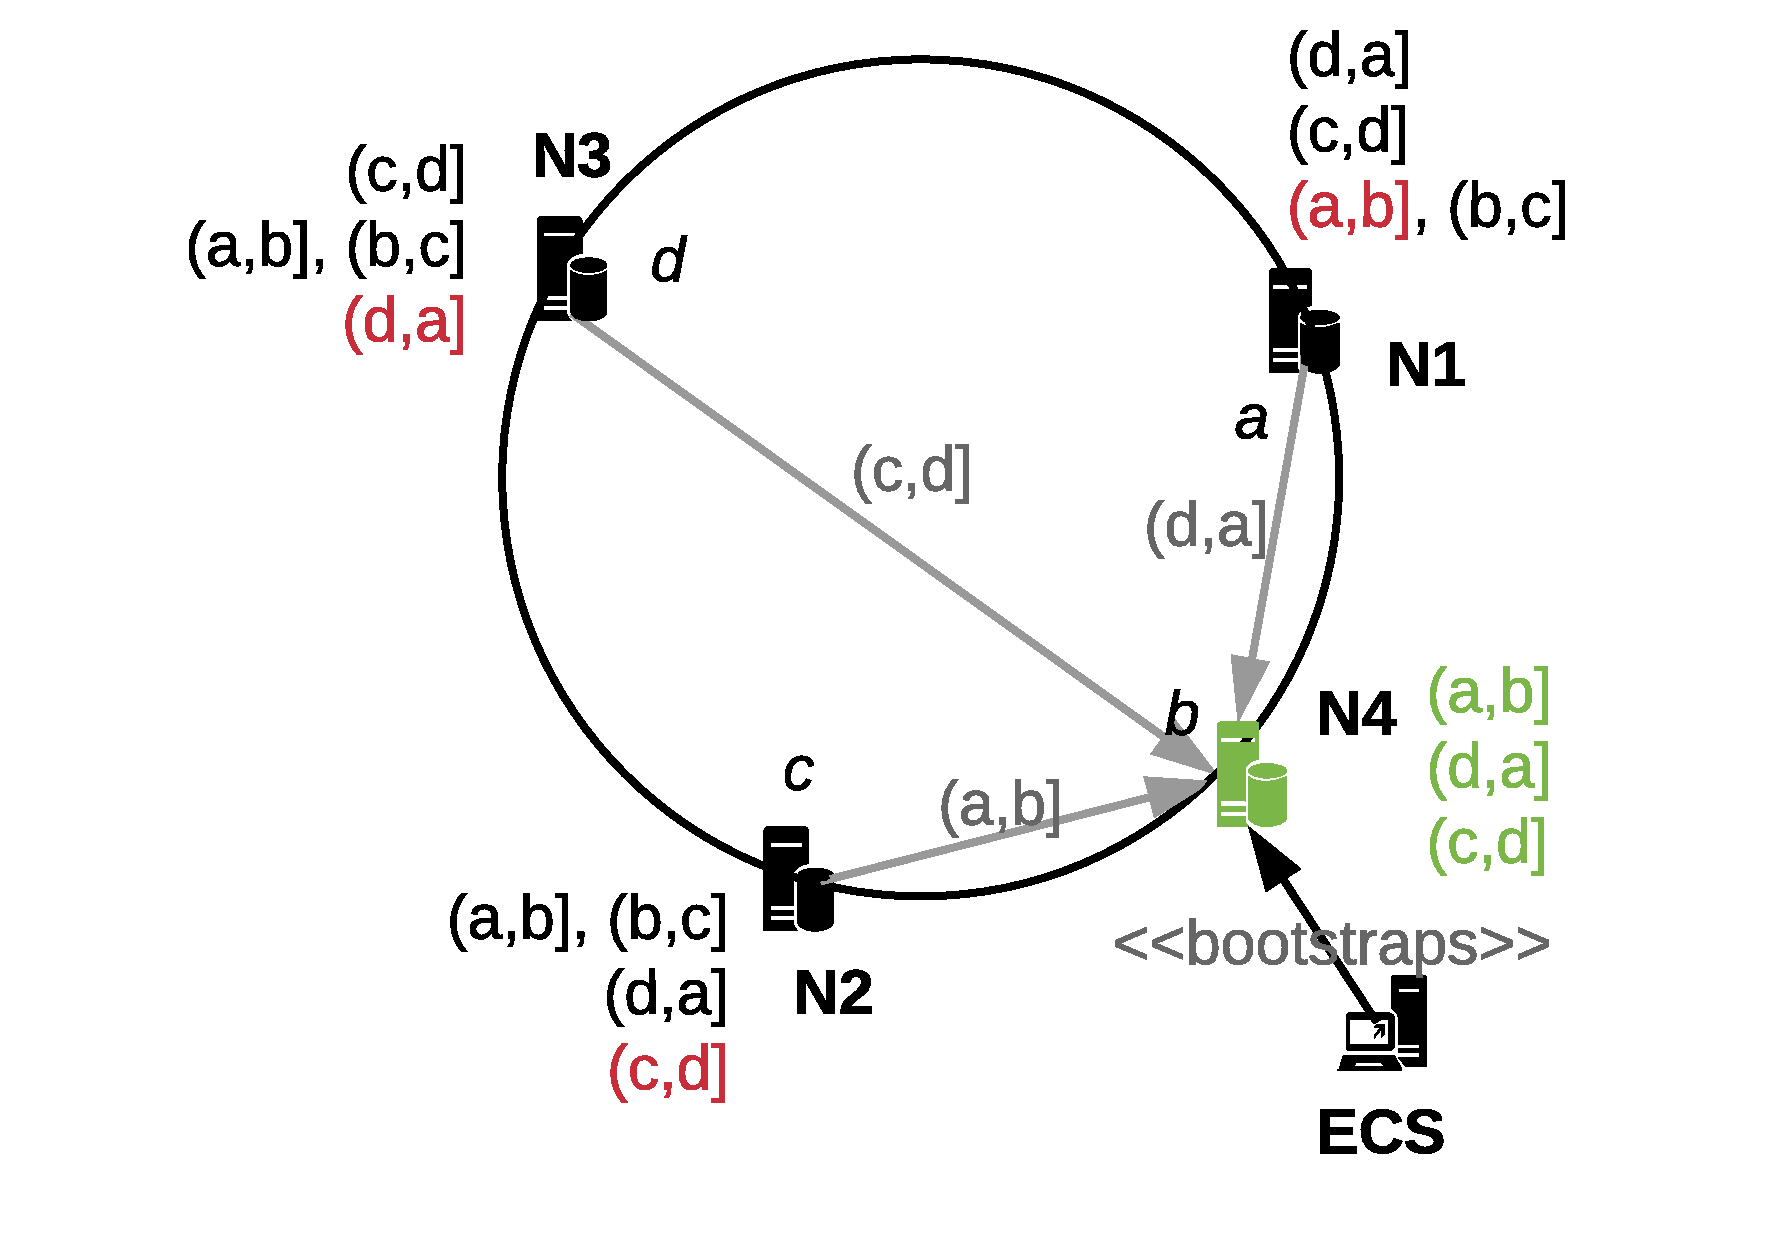
\includegraphics[width=0.4\textwidth]{resources/add-node}
	\caption{Membership - Adding a Node}
	\label{fig:add-node}
	{
	Node 4 is added at ring position $b$.
	Next to a node are the key ranges in its responsibility, assuming a replication factor of 3.
	N4's synchronization engine will initiate data stream tasks (gray arrows) to obtain the green key ranges.
	Red ranges will be cleaned up at some point.
	}
\end{figure}

Adding a node to the cluster is initiated via the \ac{ecs}. The \ac{ecs} connects
to the physical node and starts a G4DB instance.
The started instance receives the addresses of some other cluster members and starts
Gossiping-rounds announcing its arrival.
Two things happen in parallel:
Firstly, each impacted predecessor switches the corresponding replication target to the new node.
Secondly, the new node initiates data streams to obtain the data ranges for which it will be
responsible after joining (cf. Figure~\ref{fig:add-node}).
As soon a source node starts streaming, it activates a write lock to avoid data inconsistencies.
After all data streams have completed, the new node changes its state to signal that it
successfully joined the cluster.
When other nodes receive this information, they reevaluate their responsibilities and start
handling client requests accordingly.

% TODO clean up

\subsubsection{Removing Nodes}
\label{sec:remove-node}

\begin{figure}[]
	\centering
	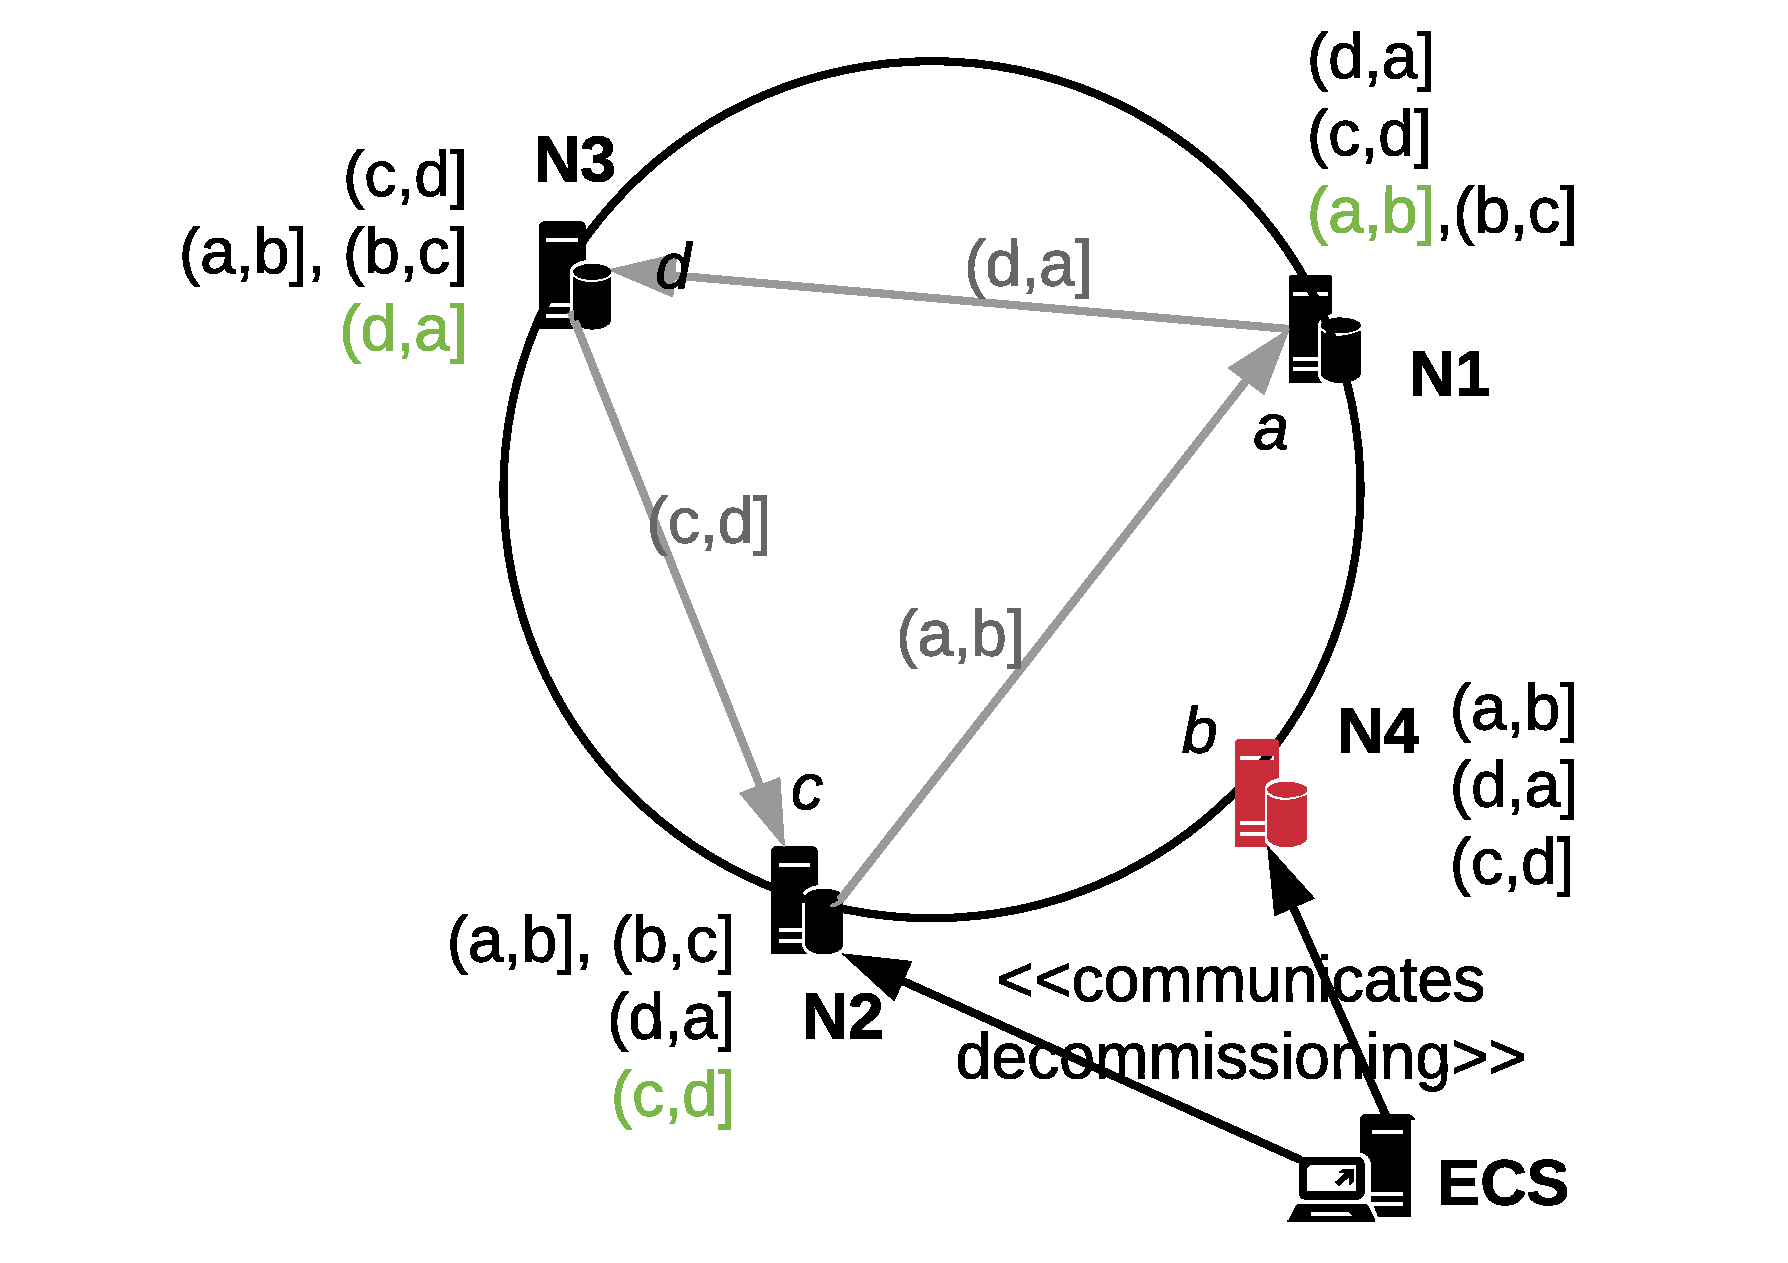
\includegraphics[width=0.4\textwidth]{resources/remove-node}
	\caption{Membership - Removing a Node}
	\label{fig:remove-node}
	{
	Node 4 is removed again.
	The synchronization engines of all impacted nodes will initiate data stream tasks (gray arrows) to obtain the green key ranges.
	}
\end{figure}

The removal of a node can either be triggered manually by an administrator
or by the failure detector when a node is believed to have failed.
In both cases the process is triggered by the \ac{ecs}.
It changes the status of the node to decommissioned and seeds that status
into the cluster.
If the decommissioned node is still alive and receives this status update, it
shuts down immediately.
The neighbors of this node become responsible for additional data partitions
due to the decommissioning.
As soon they receive the updated status, they initiate the acquisition of
such partitions which they do not already posses (cf. Figure~\ref{fig:remove-node}).

G4DB it its current version uses the same mechanism to remove nodes, regardless if
they are removed due to orderly downscaling or because of a failure-scenario.
This means that even in the case of an orderly downscaling, the replication factor
temporarily decreases.
This could be avoided in future developments by implementing
an orderly hand-off mechanism.

\subsubsection{Failure Detection}
G4DB's failure detection mechanism is currently implemented in a centralized fashion.
The \ac{ecs} continuously samples the cluster state from a small number of nodes
and keeps track of the last time it has seen a status update for each node.
Gossip messages contain a monotonically increasing heartbeat for this reason,
and only a node itself will update its heartbeat.
Therefore a node has likely crashed or is not reachable anymore if no
messages with updated heartbeats disseminate through the cluster.
If \ac{ecs} does not observe updated heartbeats for a node for a specified
amount of time, it triggers the decommissioning process for this node and
then commissions a replacement.

This is a simple \emph{accrual failure detection} mechanism which does not
adapt itself to changing network conditions.
Updating to the Phi Accrual failure
detection mechanism described by Hayashibara and colleagues~\cite{Hayashibara2004} could be a next step in the development of G4DB.
Also the failure detection mechanism should be moved out of the \ac{ecs} and into the cluster,
e.g. by using a ring-based topology.

\subsection{MapReduce}

MapReduce is a programming model for data processing that originates from
functional programming.
It was discovered by Google engineers to provide a powerful abstraction for writing
distributed and failure-tolerant data processing programs.
The developer implementing a MapReduce-program specifies two functions:

\begin{description}
	\item [\texttt{map}:] \texttt{(k1, v1) -> list((k2, v2))}
	\item [\texttt{reduce}:] \texttt{(k2, list(v2)) -> v2}
\end{description}

MapReduce is a batch-processing model.
One processing stage proceeds as follows (cf.~\cite{Laemmel2008}), where 
meaninful processing pipelines can comprise several stages that build upon
each others' results.

\begin{enumerate}
	\item The original data records are iterated over, the \texttt{map}-function
		is applied to each and produces one or more intermediate data tuples.
	\item The intermediate tuples are grouped by their respective keys.
	\item Each group is reduced to a single, aggregated value using the \texttt{reduce}-function. 	
\end{enumerate}

It is important to note that the \texttt{map}-operation can be parallelized
completely while the \texttt{reduce}-operation can be parallelized for
different keys.

\subsubsection{Topology}
All relevant parts of a MapReduce-process happen on server-side, the client is
not involved after a job has been started.
A process comprises one master for the whole cluster and one worker per node.

\subsubsection{Interaction}
The client triggers a MapReduce-job via the \acs{api}.
The request contains the user script defining the \texttt{map}- and \texttt{reduce}-functions.  
The node which receives this script starts a master process.
The master process creates a plan defining which node will process which data partition and federates the job request accordingly.
Typically each node will process its primary partition, but this could differ in cases of fail-over. 
Each node starts a worker process when it receives the federated request.
The worker process starts applying the user script on the data range specified in the request.
Each worker eventually sends back its pre-reduced results to the master process.
The master process executes one additional reduction upon receiving each worker result
in order to combine them.
The final result is stored in the cluster using the normal key distribution strategy.

\subsubsection{Worker Fail-Over}
If the master process does not receive the result from a worker within a certain
amount of time, it will poll this worker to check if it is still processing data.
If the polled node encountered an error or is not reachable, the master retriggers
the processing for the corresponding data partition on one of the replica nodes.

It shall be mentioned at this point that the master process is a single point of failure and bottleneck
in the current implementation.
We will talk more about this in Section~\ref{sec:conclusion}.


\section{Implementation}
\label{sec:implementation}
% only interesting aspects

\subsection{Architecture}

\begin{figure}[]
	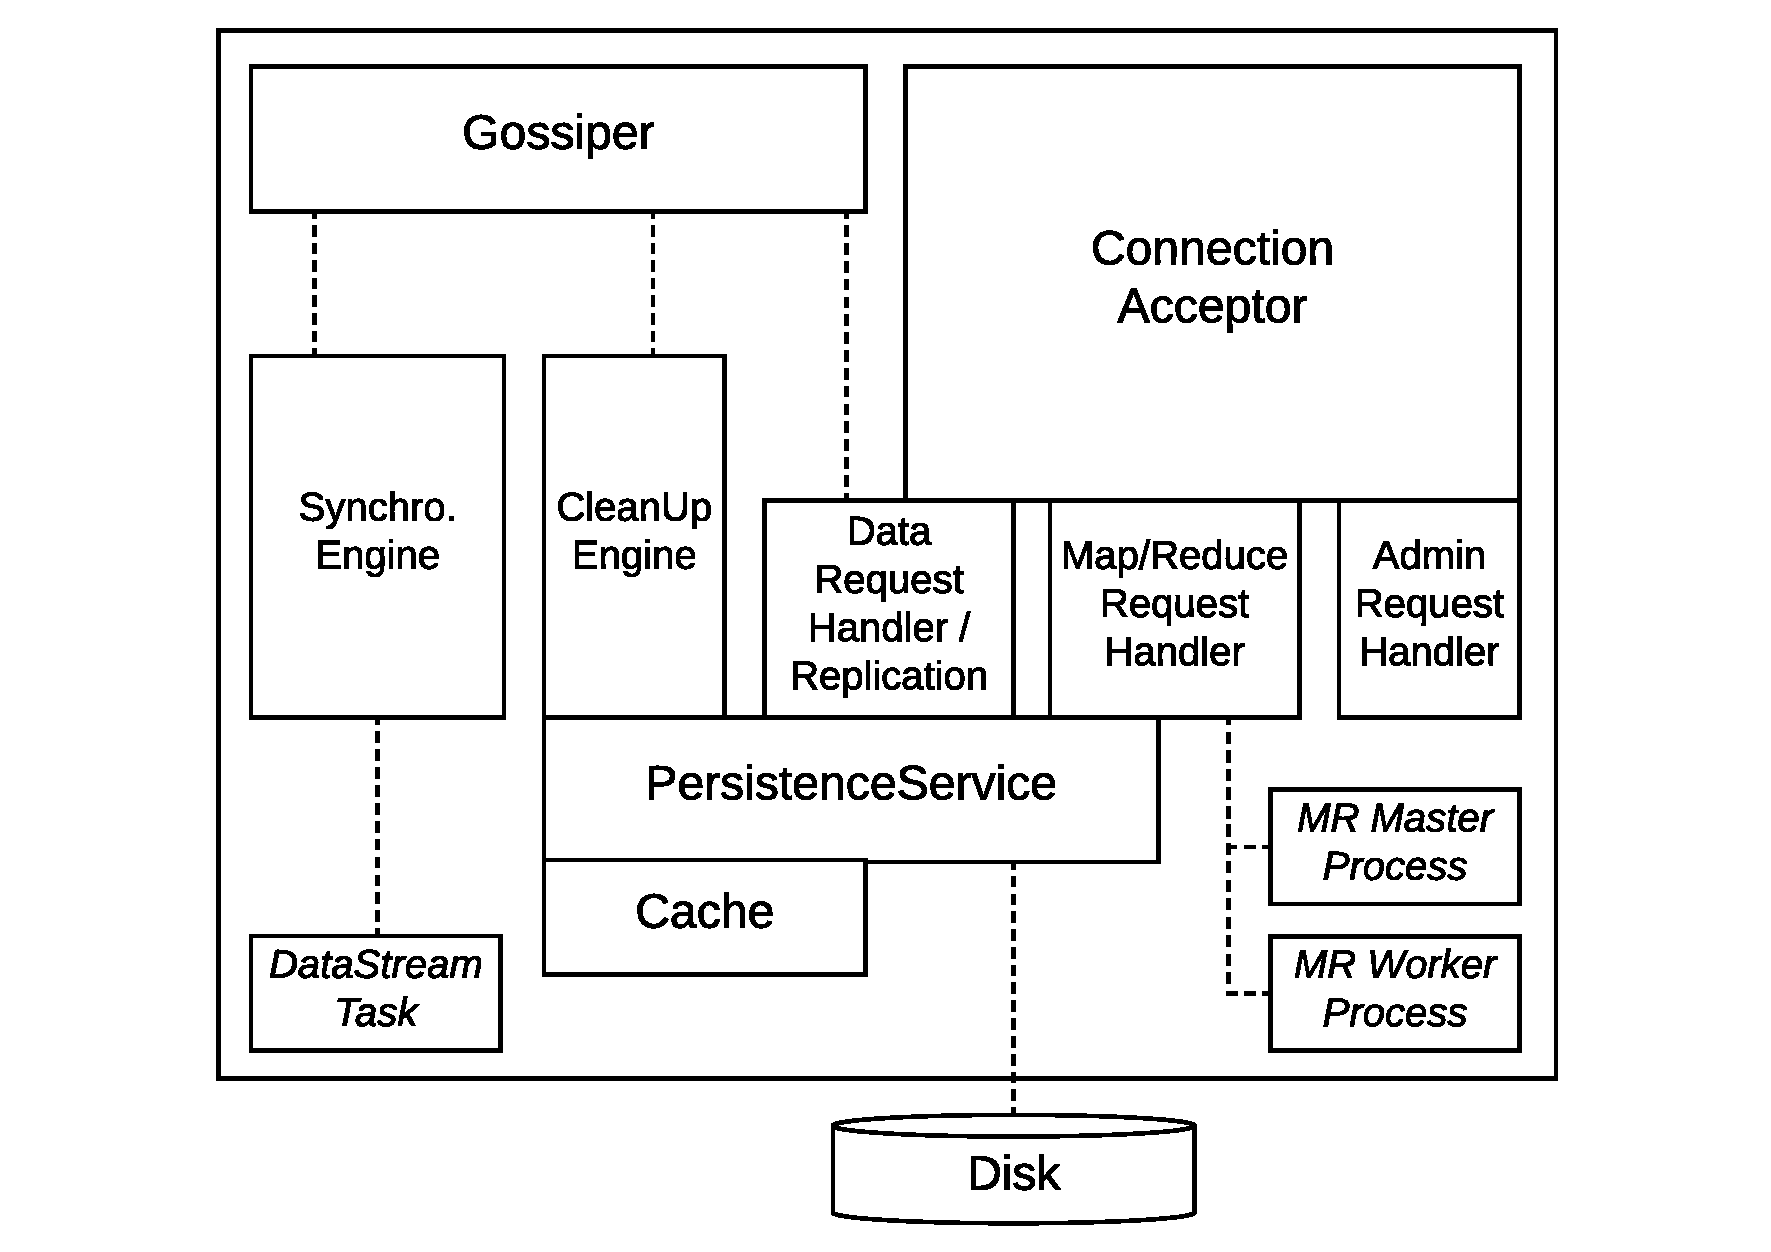
\includegraphics[width=\linewidth]{resources/architecture}
	\caption{Architectural Overview}
	\label{fig:arch}
\end{figure}

The implementation of G4DB conceptually comprises several high-level modules (cf.~Figure~\ref{fig:arch}).
Their responsibilities are as follows.

\begin{description}
\item[Connection Acceptor] Handles all incoming network communication from clients and peer nodes.
\item[Data Request Handler] Handles \texttt{PUT}/\texttt{GET} requests and takes care of replication.
\item[Map/Reduce Request Handler] Handles all MapReduce-related requests, initiates and maintains master and worker processes.
\item[Admin Request Handler] Handles administrative requests from the \ac{ecs}.
\item[Gossiper] Executes the Gossip-based membership coordination.
\item[Synchronization Engine] Coordinates the reallocation of data when nodes join or leave the cluster.
\item[CleanUp Engine] Cleans up data for which a node lost responsibility due to cluster changes.
\item[Persistence Service] Responsible for data persistence and caching.
\end{description}


\subsection{Local Persistence}
% one file per record
The persistence layer of G4DB stores each key-value-pair in a separate file.
This allows accessing data with minimal synchronization costs.
Data is cached for reading, cache size and displacement strategy are configurable.
G4DB provides \ac{fifo}, \ac{lfu} and \ac{lru} caches.
All cache implementations provide $O(1)$ performance for both store and read operations~\cite{Malike2017, Ketan2010}.
Writes are not cached and write operations are only considered successful when the data has been written to disk.
This limits write performance, but ensures that successful writes are not lost when a node crashes.
We will talk about approaches to improve the performance of the persistence layer in Section~\ref{sec:conclusion}.

\subsection{Network Protocol}
% simple layered ASCII-based
The wire protocol of G4DB is ASCII-based.
This induces some overhead compared to a binary protocol both in processing time and network traffic,
but we deem this overhead acceptable for our usecase (cf. \cite{Azad2017}).
The benefits are less complex parsing logic and simplified debugging.

\subsection{Gossiping}
% selection of nodes
% data structure
% merging strategy
\subsubsection{Peer Selection}
\label{sec:implementation:gossip:peers}
A G4DB node initiates a Gossiping-round every second and chooses between 1 to 3 peers using the following process:

\begin{enumerate}
	\item One random node is chosen from the whole cluster.
	\item One of the seed nodes is added probabilistically with a chance of 30\%.
		This aims at promoting the seed nodes to hotspots for the distribution of recent updates
		and thereby reducing dissemination time.
	\item One of the nodes believed as dead, i.e. one that has not replied in an earlier round, is added
		probabilistically with a chance of 30\%.
		This aims at reevaluating node states timely after communication problems.
\end{enumerate}

\begin{figure}[]
	\centering
	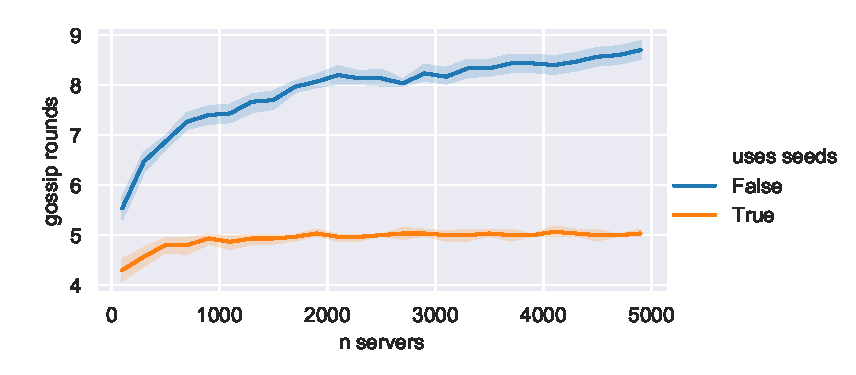
\includegraphics[width=\linewidth]{resources/gossip_scaling}
	\caption{Scalability of Gossip-Communication}
	\label{fig:perf:gossip}
	{
	Number of Gossiping-rounds necessary for a message to completely disseminate
	through the cluster dependent on the number of nodes.
	In the first experiment, 1 peer is chosen in each gossiping round (blue plot).
	In the second experiment, one of 3 seed nodes is added probabilistically with a chance
	of 30\% to the chosen random node (orange plot).
	Shaded areas denote 95\% confidence intervals.
	}
\end{figure}

We have conducted a simulation to get a feeling for how many rounds of gossip it takes
for a message to disseminate through the cluster.
We have found that this time stays in reasonable bounds even for larger number of nodes (cf. Figure~\ref{fig:perf:gossip}).

\subsubsection{Message Structure}

The structure of the Gossip messages is modeled after Cassandra (cf. \cite{Brown2014}).
It contains a status for each (known) node in the cluster.
A node status comprises following fields:

\begin{table}[H]
	\begin{tabular}{@{}lp{2.5in}@{}}
		\toprule
		Field                & Description                                               \\ \midrule
		Generation           & Local timestamp set when a node starts.                                   \\
		Heartbeat            & Updated regularly by the node.                                    \\
		State                & One of \texttt{STOPPED}, \texttt{OK}, \texttt{REBALANCING}, \texttt{JOINING}, \texttt{DECOMMISSIONED}. \\
		State Version        & Counter that is updated every time the state is updated.  \\ \bottomrule
	\end{tabular}%
\end{table}

\subsubsection{Communication Pattern}

A Gossiping-round comprises a single request-response cycle between the initiator and
each of its chosen peers.
The initiator sends its full view of the cluster to the peer, the peer merges it with
its own state and sends the updated state back to the initiator.
The initiator than merges the received state back into its own state.
Compared to Cassandra's three-way communication pattern this produces more network traffic
since the full cluster state is send along with each message.
As a benefit the implementation is more straightforward.

\subsubsection{State Merging}

During a Gossip-exchange both peers will typically have data about the same nodes.
The merged state should only contain the more recent information.
Recency is determined by state attributes in following order:

\begin{enumerate}
	\item \emph{Generation}: If one entry has a newer generation time, this means
		the node has been restarted and all old information is obsolete.
	\item \emph{State version}: The main reason to check the state version is node decommissioning.
		The \ac{ecs} seeds an updated node state with state \texttt{DECOMMISSIONED} and incremented
		state version into the cluster.
		If the impacted node is still alive and receives such a message, it will take on the decommissioned status and shutdown immediately.
	\item \emph{Heartbeat} All other things being equal, the state with the more recent heartbeat wins. 
\end{enumerate}

\subsection{MapReduce}

\subsubsection{Master Placement}
The MapReduce-\acs{api} requires the client to come up with a unique ID.
This allows G4DB to deterministically associate a MapReduce-job with a certain cluster node using the same
consistent hashing mechanism that is used for data records.
Like this, masters can be distributed across the cluster while
the client remains capable of locating it, e.g. for polling the status after reconnecting.

\subsubsection{Processing}

Mapping and reducing are not executed sequentially but in a pipelined fashion in order
to reduce memory consumption on the nodes.
More specifically, there is a configurable buffer size per key.
Once the number of mapped records exceeds this buffer size, a reduce operation is executed.
After all records have been mapped, a final worker-side reduce is executed in order
to have only one result per key.
These results are then sent back to the master where results of different workers
are combined using the same reduction logic.

The shuffle-phase happens implicitely in memory while mapped records are encountered.
There is currently no mechanism to spill intermediate data to disk, which means that MapReduce-programs
generating a large number of mapped keys will cause memory problems.


\subsubsection{Scripting}
The MapReduce-engine employs the Nashorn JavaScript engine \cite{Nashorn} included
with the JDK for user scripts.
It implements the ECMAScript~5.1~\cite{Ecma} standard including additional
extensions (cf.~\cite{Nashorn2}).


% master on one node
% workers on all nodes
% reduction on workers to save network traffic
% 2nd reduction on master
% failover for workers
% limitations: no master fail-over, no huge reduced key-set

\section{Evaluation}
\label{sec:evaluation}

\subsection{Read/Write Performance}

\begin{figure}
	\centering
	\begin{minipage}{.45\linewidth}
		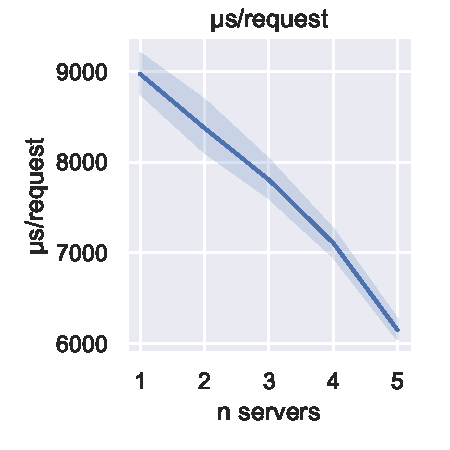
\includegraphics[width=\linewidth]{resources/servers_micros_request}
	\end{minipage}
	\hspace{0.05\linewidth}
	\begin{minipage}{.45\linewidth}
		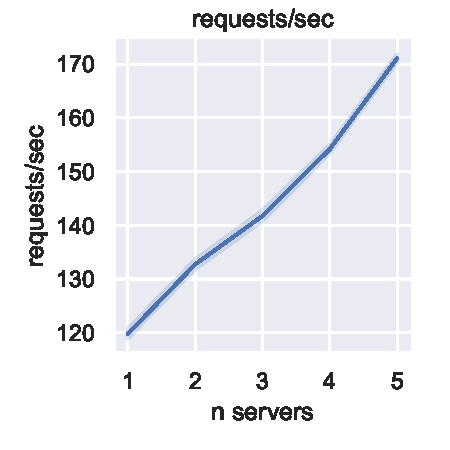
\includegraphics[width=\linewidth]{resources/servers_requests_sec}
	\end{minipage}
	\caption{Latency-related Performance Characteristics}
	{Payload size is 10kB.
	Shaded areas indicate 95\% confidence intervals.}
	\label{fig:perf:latency}
\end{figure}

\begin{figure}
	\centering
	\begin{minipage}{.45\linewidth}
		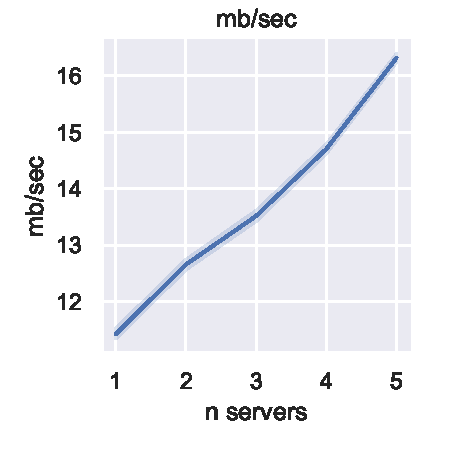
\includegraphics[width=\linewidth]{resources/servers_mb_sec}
	\end{minipage}
	\hspace{0.05\linewidth}
	\begin{minipage}{.45\linewidth}
		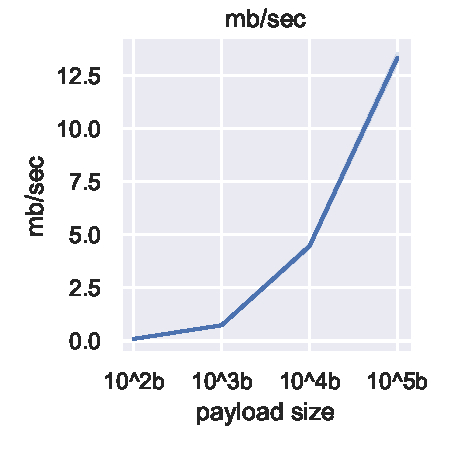
\includegraphics[width=\linewidth]{resources/payload_mb_sec}
	\end{minipage}
	\caption{Throughput-related performance characteristics}
	{Payload size in the left chart is 10kB. Shaded areas indicate 95\% confidence intervals.}
	\label{fig:perf:throughput}
\end{figure}

We conducted the performance measurements for G4DB on a Google Cloud cluster with 5 nodes as servers and 3 nodes as clients.
The nodes are n1-standard-1 instances with one 2.6GHz Xeon Core, 4GB RAM, 1000MBit network and non-SSD disks.
As general setup for latency- and throughput-related performance measurements we have 3 clients writing synthetic
records of fixed size to a G4DB cluster with a varying number of nodes.

We find that write performance increases linearly with the number of server nodes (cf.~Figure~\ref{fig:perf:latency}).
This validates G4DB's design for scalability.
As another interesting insight, we find that the throughput increases significantly when we increase message payload (cf.~Figure~\ref{fig:perf:throughput}).
There are two likely explanations for this:
Firstly, increased message payload reduces protocol overhead.
Secondly, our persistence implementation currently is unbuffered and involves random rather than sequential disk access,
which makes write operations expensive. We talk about avenues for improvement in Section~\ref{sec:conclusion}.

We do not talk about read-performance in this report, since this is a more complex topic which depends on use case and cache configuration.
We found the read-performance to be between 5-10MB/s given 10kB messages.

\subsection{MapReduce Performance}

%\begin{listing}
%	\inputminted[fontsize=\footnotesize,breaklines]{JavaScript}{sales_by_country.js}
%	\caption{MapReduce - Aggregating Sales by Country}
%	\label{lst:mr}
%\end{listing}

To evaluate our MapReduce-implementation, we look at a simple use case of aggregating sales volume by country. % (cf.~Listing~\ref{lst:mr}).
We use the online retail data set compiled by Daqing Chen and colleagues~\cite{Chen2012}.
We conducted minimal preprocessing to transform the data set from normalized CSV-format to a \ac{json}-encoded
version more suitable for a key-value-store.
We also duplicated it 15 times to reach a more significant size of 397,000 records (1.9GB).

We had to slightly manipulate G4DB to simulate an approximately uniform distribution of data across nodes,
but have then be able to process the data in approximately 5s with 10 nodes (cf.~Figure~\ref{fig:perf:mr}).


%
%\footnotetext{Such linear behaviour should be expected in real-world settings only under two conditions:
%Firstly, the read and write requests should target the whole key-range uniformly.
%Secondly, the cluster nodes should be responsible for comparable parts of the key range.
%The second condition might often not be fulfilled with a small number of nodes.}

\begin{figure}[]
	\centering
	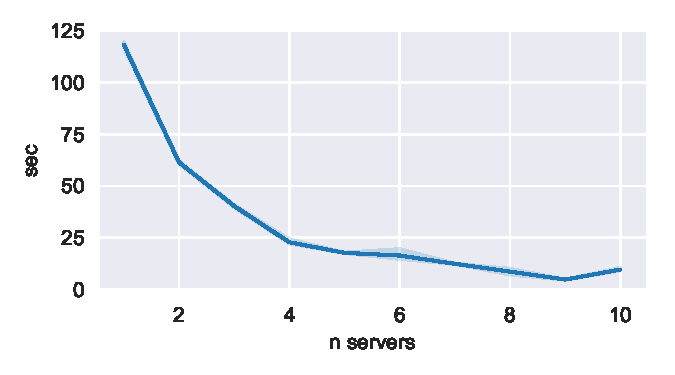
\includegraphics[width=0.8\linewidth]{resources/mr_sim}
	\caption{Performance of MapReduce}
	\label{fig:perf:mr}
	{
	Time necessary to aggregate sales by country for 397,000 records.
	Shaded areas denote 95\% confidence intervals.
	The fluctuation at the end hints at a situation where the data
	a single node has to process becomes so small that the network
	communication overhead exceeds the actual processing time.
	}
\end{figure}

\section{Conclusion}
\label{sec:conclusion}

We have designed and implemented G4DB, a highly scalable, failure-tolerant and
widely applicable key-value-datastore with integrated MapReduce-functionality.\\[1em]

The current state of implementation should be seen as a proof-of-concept
and there are many areas future developments could improve upon.

In Section~\ref{sec:evaluation} we already hinted at the inefficiencies of the
currently rather primitive implementations of network protocol and persistence layer.

The protocol could be replaced with a optimized binary version to reduce
some network traffic and decoding overhead.
Since G4DB is designed to work with textual data, the savings by doing so
should be expected to be rather marginal.
More interesting avenues for the network communication could be adding compression
and bulk requests that reduce network overhead.

The disk persistence currently uses one file per value and does not buffer writes to disk,
i.e. a write is only reported as successful when the file has been written to disk.
While this reduces the chances for data loss in case of failures, it is very inefficient.
Huge benefits could be gained by employing a combination
of append-only \acf{wal} and \acp{lsm} \cite{ONeil1996}.\\[1em]

The current MapReduce-implementation has a couple of scalability-related problems.
Right now, the master process is responsible both for federating
the original request to all nodes in the cluster as well as for consolidating
the responses of all nodes.
This makes it a bottle neck.

Instead of letting the master federate the request to all nodes,
it could make sense to employ the Gossiping-mechanism.
However it is not a good choice to distribute the user scripts,
since including them in all Gossip-communication would blow up the
network traffic significantly.
An idea could be making each server that was "infected" by the message
pull the script from the server it received the information from and then
immediatly make it serve requests on its own.
Secondly, a pruning mechanism for the Gossip mechanism
should be implemented if it is used to exchange more information, such that
outdated information does not accumulate.

For the consolidation of the worker results, a better approach
would be letting each node process the results for the keys
it has to store in the end.
Challenges that come with this are making sure that
replication is taken care of and additional status communication
to detect when a job has finished.

